\IfFileExists{aims.cls}{\documentclass{aims}}{\documentclass[11pt]{article}}

%%%%%%%%%%%%%%%%%%%%%%%%%%%%%%%%%%%%%%%%%%
\usepackage{amssymb} 
\usepackage{amsmath}
\usepackage{amsthm}
\usepackage{txfonts}

\def\typeofarticle{Research article}
\def\currentvolume{10}
\def\currentissue{5}
\def\currentyear{2025}
\def\currentmonth{Received date 1 July 2016, Accepted date 6 September}
\def\ppages{xxx--xxx.}
\def\DOI{ 10.3934/math.2025xxx}
\def\Received{12 December 2024}
\def\Revised{24 April 2025}
\def\Accepted{09 May 2025}
\def\Published{xx May 2025}


\numberwithin{equation}{section}
\DeclareMathOperator*{\essinf}{ess\,inf}
\makeatletter
\renewcommand{\@biblabel}[1]{#1\hfill \hspace{-0.2cm}}
\makeatother


\newcommand{\ep}{\varepsilon}
\newcommand{\eps}[1]{{#1}_{\varepsilon}}
% Español y compatibilidad de acentos
\usepackage[T1]{fontenc}
\usepackage[utf8]{inputenc}
\usepackage[spanish]{babel}
\addto\captionsspanish{\renewcommand{\proofname}{Demostración}}
% Desactivar inclusión de imágenes para compilar sin ficheros gráficos
\usepackage{graphicx}
\usepackage{float}
\makeatletter
\@ifundefined{includegraphics}{% si no está definido, no hacer nada
  \newcommand{\includegraphics}[2][]{% omitido
  }% 
}{% si está definido por graphicx, lo anulamos
  \renewcommand{\includegraphics}[2][]{% omitido
  }%
}
\makeatother


% Definir estilos de teorema primero
\newtheoremstyle{thmstyleone}{\topsep}{\topsep}{\itshape}{}{\bfseries}{.}{ }{}
\newtheoremstyle{thmstyletwo}{\topsep}{\topsep}{}{}{\bfseries}{.}{ }{}
\newtheoremstyle{thmstylethree}{\topsep}{\topsep}{}{}{\bfseries}{.}{ }{}

\theoremstyle{thmstyleone}%
\newtheorem{theorem}{Teorema}%  meant for continuous numbers
%%\newtheorem{theorem}{Theorem}[section]% meant for sectionwise numbers
%% optional argument [theorem] produces theorem numbering sequence instead of independent numbers for Proposition
%\newtheorem{proposition}[theorem]{Proposition}% 
%\newtheorem{corollary}[theorem]{Corollary}
\newtheorem{proposition}{Proposición}% to get separate numbers for theorem and proposition etc.
\newtheorem{corollary}{Corolario}

\theoremstyle{thmstyletwo}%
\newtheorem{example}{Ejemplo}%
\newtheorem{remark}{Observación}
%

\theoremstyle{thmstylethree}%
\newtheorem{definition}{Definición}%

\newcommand{\Den}{\mathop{\rm Den}}
\newcommand{\Num}{\mathop{\rm Num}}

\usepackage{cite}
\usepackage{hyperref}
% Fallbacks si no se usa la clase AIMS
\makeatletter
\@ifundefined{shortauthors}{\newcommand{\shortauthors}[1]{}}{}
\@ifundefined{address}{\newcommand{\address}[1]{}}{}
\@ifundefined{corraddr}{\newcommand{\corraddr}[1]{}}{}
\@ifundefined{keywords}{\newcommand{\keywords}[1]{\par\noindent\textbf{Palabras clave: }#1\par}}{}
\makeatother
% Enlaces DOI si la clase no los define
\providecommand{\doilink}[1]{\href{#1}{#1}}
\hyphenpenalty=10000
\setcounter{page}{1}
\setlength{\parindent}{2em}

\begin{document}

\title{El método de Schr\"oder y el punto en el infinito}

\author{%
 V{\'\i}ctor Galilea 
%  First name Last name\affil{2}
  y
Jos\'e Manuel Guti\'errez\corrauth
}

% \shortauthors is used in copyright information in the end of the paper
\shortauthors{los autores}

\address{%
{Department of Mathematics and Computer Sciences, Universidad de La Rioja, C/ Madre de Dios, 53, Logro\~no, 26006, La Rioja, Spain}}
%  \addr{\affilnum{2}}{Affiliation}}

% corresponding author
\corraddr{Email: jmguti@unirioja.es.% Tel: +1-111-111-1111;\\ Fax: +1-111-111-1111.
}

\begin{abstract}
Este trabajo presenta una investigación inicial sobre las propiedades dinámicas de un conocido método iterativo para resolver ecuaciones no lineales: el método de Schröder. Caracterizamos el grado de la aplicación racional inducida al aplicar el método a ecuaciones polinómicas, junto con otras características dinámicas como la naturaleza de los puntos fijos extraños y la presencia de ciclos atractores. Se presta especial atención a las diferencias dinámicas relevantes entre el método de Schröder y otros métodos iterativos, en particular el método de Newton, con foco en el comportamiento en el infinito.
\end{abstract}

\keywords{
{dinámica compleja; métodos numéricos; método de Newton; método de Schr\"oder; punto en el infinito}
\newline
\textbf{Mathematics Subject Classification:} 37F10, 65S05}

\maketitle


\section{Introducción}
El método de Schr\"oder es un procedimiento iterativo bien conocido para resolver ecuaciones no lineales, introducido originalmente por E. Schr\"oder en 1870 (véase \cite{1Sch} o \cite{2Stw}). Aunque el método es aplicable a una amplia clase de ecuaciones no lineales, nos restringimos a su aplicación a ecuaciones polinómicas definidas sobre el plano complejo.
\begin{equation}\label{eq1}
p(z)=0,\quad z\in\mathbb{C}.
\end{equation}

In fact, Schr\"oder's method for solving \eqref{eq1} defines a one-step nonlinear recurrence relation
$z_{n+1}=S_p(z_n)$, $n\ge 0$, given by the iteration map
\begin{equation}\label{eq2}
S_p(z)=z -\left( \frac{1}{1-  L_p(z)}\right) \frac{p(z)}{p'(z)}, 
\end{equation}
donde $L_p(z)$ se define mediante el cociente
\begin{equation}\label{eq3}
L_p(z)= \frac{p(z)p''(z)}{p'(z)^2}.
\end{equation}

El cociente definido en \eqref{eq3}, junto con sus generalizaciones a dimensiones superiores y a espacios de Banach, desempeña un papel central tanto en la formulación concisa de diversos métodos iterativos como en el análisis de sus propiedades de convergencia. Uno de los primeros trabajos que subraya la relevancia de este cociente —conocido como grado de convexidad logarítmica— es \cite{2Her}.

Originalmente, el método de Schröder se concibió como una modificación del método de Newton destinada a lograr convergencia cuadrática incluso en presencia de raíces múltiples. Es inmediato comprobar que el método se obtiene aplicando el método de Newton a la función racional $p(z)/p'(z)$. En resumen, puede decirse que el elevado coste computacional del método de Schr\"oder (en general, los métodos que usan segundas derivadas tienen orden de convergencia cúbico \cite{3Traub}) se compensa con su robustez para el cálculo de raíces múltiples. Quizá debido a esta complejidad computacional, el comportamiento dinámico del método de Schröder no ha sido estudiado de forma extensa. Con todo, creemos que el estudio dinámico de diversos métodos iterativos es valioso en sí mismo, pues puede revelar comportamientos que difieren significativamente de los mostrados por el método más estudiado: el de Newton. Por ejemplo, tales diferencias se han documentado en el caso del método de Halley \cite{4Roberts} y del método de Chebyshev \cite{5GV}. El comportamiento dinámico de los métodos iterativos, incluso en los casos más simples, proporciona información valiosa sobre la estabilidad y la convergencia global del método considerado \cite{6BCT}. El método de Schr\"oder es un tema de investigación actual; a modo ilustrativo, y sin ánimo de exhaustividad, véanse las referencias recientes \cite{6CVV2024}, \cite{6MI2025}.

Pasamos ahora al análisis dinámico del método de Schröder. En \cite{1Sch}, el propio Schröder realizó una exploración inicial de la dinámica del método, específicamente para el caso $p(z)=z^2-1$. Observó que, en este caso, las aplicaciones de iteración asociadas al método de Schr\"oder, $S_p(z)$, y al método de Newton, $N_p(z)=z-p(z)/p'(z)$, son inversas entre sí, a saber
$$
S_p(z)=\frac{2}{z+\frac{1}{z}}=\frac{1}{N_p(z)}.
$$
Como consecuencia, los comportamientos dinámicos de ambos métodos están estrechamente relacionados en este caso. Schröder llevó a cabo su análisis usando coordenadas cartesianas y polares, pero sin emplear números complejos.

Usando la teoría de Cayley y aritmética compleja, el método de Schröder puede analizarse cuando se aplica a polinomios cuadráticos generales.

$$
p(z)=(z-a)(z-b), \quad a, b \in \mathbb{C}, \quad a\ne b,
$$
es conjugado, mediante la transformación de M\"obius $M(z)=(z-a)/(z-b)$, con la aplicación $R(z)=-z^2$, es decir,
$
R(z)=M\circ S_p \circ M^{-1}(z)=-z^2.
$
El conjunto de Julia de $R(z)$ es la circunferencia unidad $\{ z\in\mathbb{C}; \vert z \vert=1\}$ y la cuenca de atracción de $z=0$ es $\{ z\in\mathbb{C}; \vert z \vert<1\}$. La cuenca de atracción de $z=\infty$ es $\{ z\in\mathbb{C}; \vert z \vert>1\}$. En consecuencia, para polinomios cuadráticos generales $p(z)=(z-a)(z-b)$, el conjunto de Julia de $S_p(z)$ corresponde a la mediatriz del segmento que une las raíces $a$ y $b$. La cuenca de atracción de la raíz $z=a$ es el semiplano que contiene a $z=a$, y la cuenca de atracción de la raíz $z=b$ es el semiplano que contiene a $z=b$. Hasta este punto, no se han observado diferencias significativas entre las dinámicas del método de Newton y del método de Schröder para polinomios cuadráticos.

However, differences begin to emerge when considering polynomials of higher degree. For example, in \cite{5GV}, the authors demonstrated that it is possible to analytically characterize the basins of attraction for Schröder's method applied to polynomials with two distinct roots $a,b \in \mathbb{C}$, each with integer multiplicities $m$ and $n$, that is, $p(z)=(z-a)^m(z-b)^n$. Without loss of generality, we may assume $m\ge n$. If $J_{m,n,a,b}$ denotes the Julia set of Schröder's method applied to such polynomials, then:
\begin{itemize}
\item If $m = n$, $J_{m,n,a,b}$ is the line of points equidistant from $a$ and $b$.
\item  If $m > n \ge 1$, then $J_{m,n,a,b}$ is a circle with center $c_{m,n,a,b}$ and radius $r_{m,n,a,b}$, where
$$ 
c_{m,n,a,b}=\frac{bm^2 - an^2}{m^2-n^2}, \qquad
r_{m,n,a,b}= \frac{mn \vert a-b\vert}{m^2-n^2}.
$$
\end{itemize}

Obsérvese que, cuando $m > n \ge 1$, tanto $c_{m,n,a,b}$ como $r_{m,n,a,b}$ pueden expresarse en función del cociente $q=m/n>1$, dando lugar a
$$ 
c_{q,a,b}=\frac{bq^2 - a}{q^2-1}, \qquad
r_{q,a,b}= \frac{q \vert a-b\vert}{q^2-1}.
$$
En consecuencia, el conjunto de Julia asociado $J_{q,a,b}$ es el círculo centrado en $c_{q,a,b}$ y de radio $r_{q,a,b}$. Así, las cuencas de atracción de las raíces $a$ y $b$ dependen principalmente de las propias raíces y del cociente $q=m/n>1$, más que de las multiplicidades individuales $m$ y $n$. Además, la evolución del conjunto de Julia correspondiente (que constituye la frontera entre las cuencas de atracción) puede visualizarse como función de $q$: pasa de la mediatriz del segmento que une $a$ y $b$ (en el caso límite $q\to 1$) a circunferencias de radio decreciente que finalmente colapsan sobre la raíz $b$ cuando $q\to \infty$, puesto que $b$ tiene menor multiplicidad (véase la Figura~\ref{fig1}).

\begin{figure}[ht]%
\centering
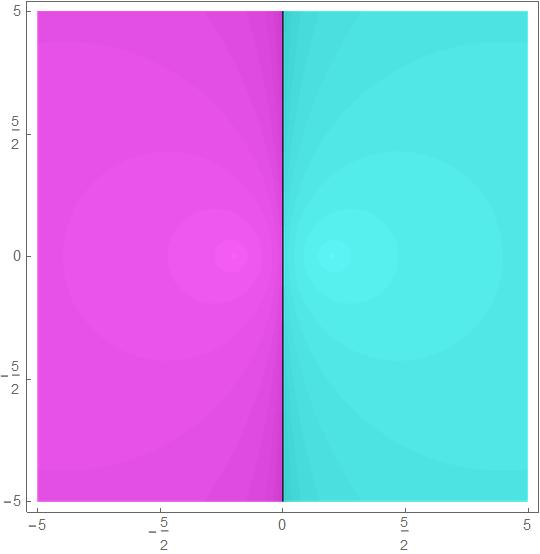
\includegraphics[height=0.33\textwidth]{img/sch_n_6_m_6.jpg}
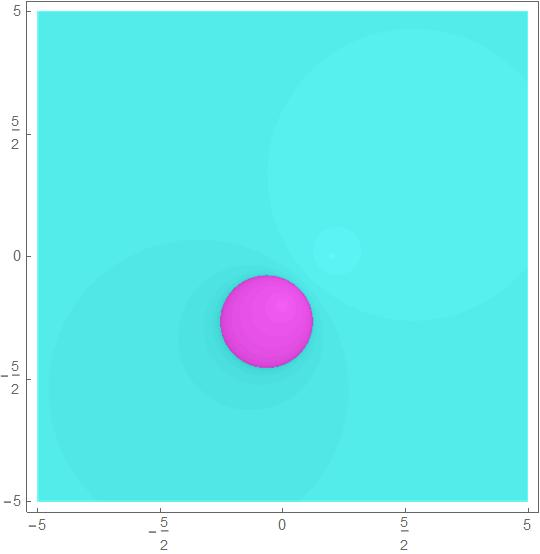
\includegraphics[height=0.33\textwidth]{img/sch-i_m2_n1.jpg}
\\[\smallskipamount]
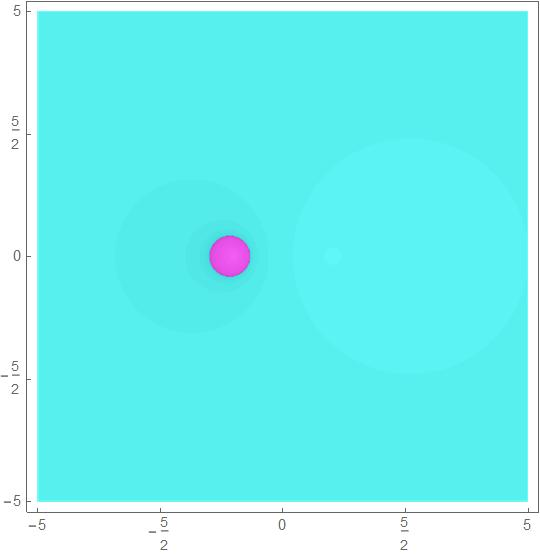
\includegraphics[height=0.33\textwidth]{img/sch_m_5n_1.jpg}
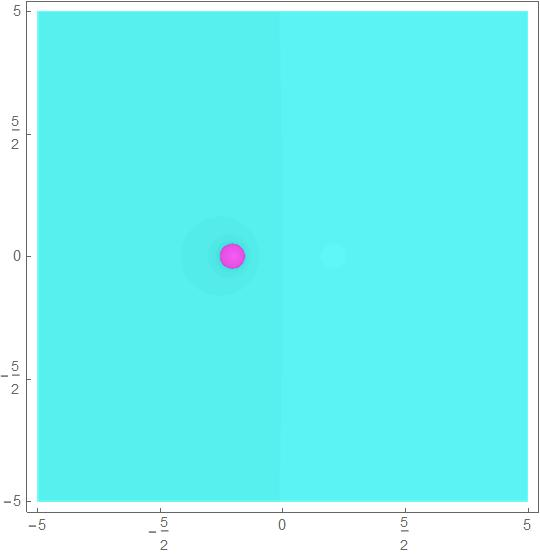
\includegraphics[height=0.33\textwidth]{img/sch_m_8n_1.jpg}

\caption{Evolución de las cuencas de atracción del método de Schr\"oder aplicado a los polinomios $p(z)=(z-1)^m(z+1)^n$ con $q=m/n$ creciente. Se muestran los casos $q=1, 2, 4, 8$ (arriba izquierda, arriba derecha, abajo izquierda y abajo derecha, respectivamente). La cuenca de la raíz $z=-1$ aparece en magenta y la de la raíz $z=1$ en cian.}\label{fig1}
\end{figure}

En el resto del artículo continuamos la investigación de propiedades destacadas del método de Schröder aplicado a polinomios. En la Sección~\ref{section2} caracterizamos el grado de la aplicación racional que surge al aplicar el método de Schröder. En la Sección~\ref{section3} mostramos que el método de Schröder admite puntos fijos extraños, todos ellos repelentes, y examinamos la posible existencia de ciclos atractores. Finalmente, en la Sección~\ref{section4} analizamos el comportamiento del infinito para la aplicación de iteración definida en \eqref{eq2}.

\section{Grado del método de Schr\"oder} \label{section2}

In the study of the dynamical behavior of iterative methods for solving polynomial equations, one of the initial steps is to determine the degree of the associated rational map. While it is relatively straightforward to establish upper bounds for this degree, computing the exact value requires the introduction of the concept of a \emph{special critical point}, as employed by Nayak and Pal \cite{7NP} in their analysis of the rational map associated with Chebyshev's method (see also \cite{8GGAxioms} for the broader Chebyshev-Halley family of methods).

\begin{definition} (Punto crítico especial) Dado un polinomio complejo $p(z)$, un punto crítico $c\in\mathbb{C}$ se denomina especial si $p(c)\ne 0$ pero $p''(c) = 0$.
\end{definition} 
Para mayor comodidad, escribimos la aplicación de iteración del método de Schr\"oder \eqref{eq2} de la forma equivalente
\begin{equation}\label{eq12}
S_p(z)=z -\frac{p(z)p'(z)}{p'(z)^2- p(z)p''(z)}.
\end{equation}


\begin{theorem}\label{Teo1}
Sea $S_p(z)$ la aplicación de iteración del método de Schr\"oder para resolver ecuaciones polinómicas, escrita como en  \eqref{eq12}. Entonces el grado de la aplicación racional $S_{p}(z)$ es
$$\deg(S_{p}(z)) =2r+s-C-2,$$
where
\begin{itemize}
\item $ r $ es el número de raíces distintas de $p(z)$.
\item $s$  es el número de puntos críticos especiales de $p(z)$.
\item $C=c_1+\cdots+c_k$  es la suma de multiplicidades de todos los puntos críticos especiales. 
\end{itemize}
\end{theorem}

\begin{proof} First we note that  $\deg(\Num(S_p(z))\le \deg(\Den(S_p(z))\le 2d-2$. In fact, for a general monic polynomial written in the way $p(z)=z^d +a_{d-1} z^{d-1} + \cdots$ it is easy to prove, after a few algebraic manipulations, that
$$ \Num(S_p(z))=zp'(z)^2-zp(z)p''(z)-p(z)p'(z)=-a_{d-1}z^{2d-2}+P_{2d-3}(z), $$
$$ \Den(S_p(z))=p'(z)^2-p(z)p''(z)=-dz^{2d-2}+Q_{2d-3}(z),$$
where $P_{2d-3}(z)$ and $Q_{2d-3}(z)$ are  polynomials of degree $2d-3$. 

Consequently, $\deg(S_p(z)\le 2d-2$. In addition,  $\deg(S_p(z)< 2d-2$ if $\Num(S_p(z))$ and $\Den(S_p(z))$ have common roots. For calculating the exact degree of $S_p(z)$,  we must just   analyze $\deg(\Den(S_p(z))$.

The proof is based on the following factorizations of the polynomials $p(z)$, $p'(z)$ and $p''(z)$:
\[
p(z)=\prod_{i=1}^m(z-\alpha_i)\prod_{j=1}^n(z-\beta_j)^{b_j},\quad b_j\ge 2,
\]
with $\deg(p)=m+B$, $B=\sum_{j=1}^n b_j.$ Taking into account that a root of $p(z)$ with a certain multiplicity $k\ge 1$ is a root of $p'(z)$ with multiplicity $k-1$ (and a similar criterion for $p''(z)$), we have
$$p'(z)=g(z)\prod_{j=1}^n(z-\beta_j)^{b_j-1},$$
$$p''(z)=h(z)\prod_{j=1}^n(z-\beta_j)^{b_j-2},$$
where $g(z)$ and $h(z)$ are polynomials that satisfy $g(\alpha_i)\ne 0$, $i=1,\dots, m$, $g(\beta_j)\ne0$ and $h(\beta_j)\ne 0$ for $j=1,\dots, n$. 
In addition, $\deg(g)=\deg(p')-B+n=m+n-1$ and the leading coefficient of $g(z)$ is $d$; $\deg(h)=\deg(p'')-B+2n=m+2n-2$ and the leading coefficient of $h(z)$ is $d(d-1)$.

 Let $\gamma_j$, $j=1,\dots, s$ be the special critical points of $p(z)$, with multiplicities $c_j$. Then the polynomials $g(z)$ and $h(z)$ can be factorized in the following way:
$$g(z)=\tilde{g}(z)\prod_{k=1}^s(z-\gamma_k)^{c_k},$$
$$h(z)=\tilde{h}(z)\prod_{k=1}^s(z-\gamma_k)^{c_k-1},$$
where $\tilde{g}(z)$ and $\tilde{h}(z)$ are polynomials that satisfy $\tilde{g}(\alpha_i)\ne 0$, $i=1,\dots, m$; $\tilde{g}(\beta_j)\ne0$ and $\tilde{h}(\beta_j)\ne 0$ for $j=1,\dots, n$; $\tilde{h}(\gamma_k)\ne 0$ for $k=1,\dots, s$.
In addition, $\deg(\tilde{g})=\deg(g)-C=m+n-C-1$ and the leading coefficient of $\tilde{g}(z)$ is $d$; $\deg(\tilde{h})=\deg(h)-C+s=m+2n-2-C+s$ and the leading coefficient of $h(z)$ is $d(d-1)$.


Therefore we can simplify the common roots in the following quotient
$$
\frac{p(z)p'(z)}{p'(z)^2- p(z)p''(z)}=\dfrac{\prod_{i=1}^m(z-\alpha_i)\prod_{j=1}^n(z-\beta_j) \prod_{k=1}^s(z-\gamma_k) \tilde{g}(z)}
{\prod_{k=1}^s(z-\gamma_k)^{(c_k+1)} \tilde{g}(z)^2-\prod_{i=1}^m(z-\alpha_i)\tilde{h}(z)}.
$$
The degree of $S_p(z)$ coincides with the denominator of the previous quotient (note that there are not more common roots between the numerator and the denominator of $S_p(z)$). Note that the leading coefficient of the polynomial in the denominator of the previous quotient
$$
\prod_{k=1}^s(z-\gamma_k)^{(c_k+1)} \tilde{g}(z)^2-\prod_{i=1}^m(z-\alpha_i)\tilde{h}(z)
$$
is $d^2-d(d-1)=d$, and its degree is
$2m+2n+s-C-2 =2r+s-C-2$,  $r=m+n$ being the number of distinct roots of $p(z)$. So, we have proved the result.
\end{proof}

\begin{corollary}\label{Cor2}
Si $p(z)$ es un polinomio sin puntos críticos especiales, entonces el grado de la aplicación racional $S_{p}(z)$ es
$2r-2,$
donde $ r $ es el número de raíces distintas de $p(z)$.
\end{corollary}

Taking into account the proof of Theorem~\ref{Teo1}, we can characterize the behavior of the infinity point for Schr\"oder's method. As we can see, it is different from the behavior for the most famous iterative processes (Newton, Halley, and Chebyshev), for which infinity is a repelling fixed point. 

\begin{corollary}\label{Cor1}
El punto en el infinito no es un punto fijo para el método de Schröder \eqref{eq2}.
\end{corollary}
\begin{proof}
Following the proof of Theorem~\ref{Teo1}, and with the same notations, we have
$$
S_p(\infty)=-\frac{a_{d-1}}{d},
$$
por lo que $\infty$ no es un punto fijo para $S_p(z)$.
\end{proof}
\section{Puntos fijos extraños y ciclos para el método de Schr\"oder} \label{section3}

La existencia de puntos fijos extraños asociados a un método iterativo para resolver una ecuación polinómica como \eqref{eq1} es un tema clásico en el análisis dinámico de estos métodos. Recordemos que los puntos fijos extraños son puntos fijos de la aplicación de iteración que no corresponden a raíces de la ecuación. Es bien sabido que el método de Newton no tiene puntos fijos extraños~\cite{3Traub}. De modo similar, el método de Halley posee únicamente puntos fijos extraños repelentes (véase \cite{9Kneisl}). En contraste, el método de Chebyshev admite puntos fijos extraños atractores, como se demuestra en \cite{5GV} y \cite{10Vrscay}, entre otros.


\begin{theorem}
Sea $S_p(z)$ la aplicación de iteración del método de Schr\"oder para resolver ecuaciones polinómicas, escrita como en \eqref{eq12}. Entonces, los puntos fijos extraños de $S_p(z)$ son soluciones de $p'(z)=0$, con $p(z)\ne0$. Todos ellos son repelentes.
\end{theorem}


\begin{proof}  Teniendo en cuenta \eqref{eq12}, los puntos fijos de $S_p(z)$ son las raíces de $p(z)$ y las soluciones de $p'(z)=0$. Entonces, los puntos fijos extraños del método de Schr\"oder son puntos $\omega\in\mathbb{C}$ tales que $p'(\omega)=0$ y $p(\omega)\ne 0$. Sea $m\in \mathbb{N}$ la multiplicidad de $\omega$ como raíz de $p'(z)$, esto es,
$$
p'(z)=(z-\omega)^m g(z),
$$
con $g(\omega)\ne 0$. Sustituyendo en \eqref{eq12}, obtenemos 
$$
S_p(z)=z -(z-\omega)H(z), \quad H(z)=\frac{p(z)g(z)}{(z-\omega)^{m+1}g(z)^2-p(z)(mg(z)+(z-\omega)g'(z))}.
$$
Ahora, teniendo en cuenta que el denominador en $H(\omega)$ no es cero, se deduce tras unas pocas manipulaciones algebraicas
$$
S'_{p}(\omega)=1-H(\omega)=1 +\frac{1}{m} >1.
$$
En consecuencia, el multiplicador de $\omega$ como punto fijo es mayor que uno, y $\omega$ es un punto fijo repelente.
\end{proof}

As discussed in the introduction, the behavior of Schröder's method for quadratic polynomials ---and more generally, for polynomials with two distinct roots--- is completely understood (see \cite{11Gali}). However, when the method is applied to polynomials of higher degree, its dynamical behavior becomes significantly more intricate. In such cases, there may exist open sets of initial guesses that fail to converge to any root of the given polynomial. Having established that Schröder's method does not possess attracting extraneous fixed points, we now focus on demonstrating the existence of attracting cycles. To this end, we employ the technique introduced by Roberts and Horgan-Kobelsky in \cite{4Roberts}. In particular, we investigate the case of cubic polynomials.

As a preliminary step, we present a useful result known as the Scaling Theorem, which allows us ---through appropriate changes of variables--- to reduce the study of the dynamics of various iterative methods, possibly involving several parameters, to simpler representative cases (see \cite{12ABP} for applications to other iterative methods).

\begin{theorem} {(Scaling Theorem for Schröder method)} Let $f$ an analytic function defined in the Riemann sphere and let $T(z)=\alpha z+\beta$ be an affine transformation. If $g(z)=f(T(z))$, we have that $T\circ S_g \circ T^{-1}=S_f$. Hence, $S_f$ and $S_g$ are topologically conjugated, where $S_f$ and $S_g$ are, respectively, Schr\"oder's iteration maps applied to $f$ and $g$.
\end{theorem}

\begin{proof}
Firstly, we calculate the composition $S_g(T^{-1}(z))$:
\begin{equation}
S_g(T^{-1}(z))=T^{-1}(z)-\frac{g(T^{-1}(z))}{g'(T^{-1}(z))}\frac{1}{1-L_g(T^{-1}(z))}.
\end{equation}
Starting from the equality $g(T^{-1}(z))=f(z)$ we have that:
$$		
f'(z)=(g \circ T^{-1})'(z)=\frac{1}{\alpha}g'(T^{-1}(z))
$$
and
$$
		f''(z)=(g \circ T^{-1})''(z)=(\frac{1}{\alpha}g'(T^{-1}(z)))'=\frac{1}{\alpha^2}g''(T^{-1}(z)).
$$
Consequently,
$$
		L_g(T^{-1}(z))=\frac{g(T^{-1}(z))g''(T^{-1}(z))}{g'(T^{-1}(z))^2}=L_f(z).
$$
Therefore:
$$	
		S_g(T^{-1}(z))=T^{-1}(z)-\frac{1}{\alpha}\frac{f(z))}{f'(z))}\frac{1}{1-L_f(z))},
$$
$$
		T(S_g(T^{-1}(z)))=\alpha(T^{-1}(z)-\frac{1}{\alpha}\frac{f(z))}{f'(z))}\frac{1}{1-L_f(z))})+\beta.
$$
As $T^{-1}(z)=(z-\beta)/\alpha$, we deduce the stated result $T(S_g(T^{-1}(z)))=S_f(z)$.
\end{proof}

The Scaling Theorem enables us to reduce the study of the dynamical behavior of Schröder's method, when applied to a general cubic polynomial, to a family of polynomials depending on a single complex parameter. One such family ---among several, all of which are topologically conjugate--- suitable for analyzing the dynamics of Schröder's iteration map for cubic polynomials is given by
\begin{equation}\label{eq4}
p_{\lambda}(z)=(z^2-1)(z-\lambda),\quad \lambda\in \mathbb{C}.
\end{equation}

Note that we can identify each polynomial in \eqref{eq4} with the corresponding complex number $\lambda\in \mathbb{C}$. So, for our convenience, we can simplify the notation employed until this moment, and we can denote by $S_{\lambda}$ the iteration map obtained by applying Schr\"oder's method  \eqref{eq2}  to a polynomial in \eqref{eq4} , that is
\begin{equation}\label{eq5}
S_{\lambda}(z)= S_{p_{\lambda}}(z)=z -\left( \frac{1}{1-  L_{p_{\lambda}}(z)}\right) \frac{{p_{\lambda}}(z)}{{p_{\lambda}}'(z)}, 
\end{equation}

 The parameter space is a powerful graphical tool that enhances our understanding of the behavior of the iteration map defined in \eqref{eq5}. It has been employed by several authors to investigate other iterative processes (see, for instance, \cite{5GV,10Vrscay,13Vrscay0}). This space is constructed by tracking the orbits of the free critical points of the corresponding iteration map. Free critical points are those critical points of a root-finding method that do not coincide with any of the roots of the polynomial equation being solved. The strategy of analyzing the orbits of critical points is grounded in the following classical theorem (see \cite{14Beardon}): 

\begin{theorem}[Fatou-Julia]
Every attracting cycle of a rational map attracts at least one critical point.
\end{theorem}

In our case, for Schr\"oder's iteration map  \eqref{eq2}, formally we have that its derivative is
$$
S'_{p}(z)=-\frac{L_p(z)-2L_p(z)^2+L_{p'}(z)L_p(z)^2}{(1-L_p(z))^2},
$$
where
 $$ L_{p'}(z)=\frac{p'(z)p'''(z)}{p''(z)^2}.$$


In particular, for polynomials in the family \eqref{eq4} and the iteration map \eqref{eq5}, to obtain the free critical points, we have to solve $S'_{p}(z)=0$. After a few algebraic manipulations and discarding the three roots of $p_{\lambda}(z)$, we obtain the cubic equation
$$
(\lambda ^2+3) z^3-12 \lambda  z^2+(9 \lambda ^2 +3) z-2 \lambda ^3-2 \lambda =0.
$$

In this case, the study of the parameter plane associated with Schröder's method applied to the family of polynomials given by \eqref{eq4} requires the numerical solution of the preceding equation. This yields three free critical points, denoted  $\rho_i$, $i=1,2,3$. This represents a key distinction from other methods ---such as Newton's, Halley's, or Chebyshev's--- where the free critical points can be computed explicitly via linear or quadratic equations. To visualize the parameter planes corresponding to Schröder's method \eqref{eq5}, a color palette with $3^3= 27$ colors would be needed to represent all possible behaviors. However, due to the complexity of such a representation, we simplify the visualization by using only two colors: Black for values of $\lambda$ where the orbit of at least one free critical point does not converge to a root, and white for values of $\lambda$ where the orbits of all free critical points converge to roots. In the latter case, this guarantees that no attractors other than the roots are present. Some details of this parameter plane are shown in Figure~\ref{fig2bis}.

\begin{figure}[H]%
\centering
\includegraphics[height=0.3\textwidth]{img/imagen_1.png}
\includegraphics[height=0.3\textwidth]{img/plano_parametros_eje_imaginario.jpg}
\includegraphics[height=0.3\textwidth]{img/imagen_5.png}
\caption{Three images of parameter plane of  Schröder's method applied to the $p_{\lambda}(z)$ family. In black the values of $\lambda$ for which at least the orbit of one of the three free critical points does not converge to any root and in white the opposite case. On the left, we have drawn the parameter plane only in the first quadrant, taking into account the double symmetry with respect to the coordinate axes. Note that this parameter plane is not connected. There are multiple Mandelbrot-like sets scattered throughout the rest of the plane. For instance, in the right figure, we show one of them, corresponding to the values around the point $3.1+2.3i$. In the midddle, a magnification around the imaginary axes.}\label{fig2bis}
\end{figure}


\section{El comportamiento del punto en el infinito en el método de Schr\"oder} \label{section4}

Si consideramos ahora el plano complejo extendido $\hat{\mathbb{C}}=\mathbb{C}\cup\{\infty\}$, el punto en el infinito puede verse como otro punto del plano complejo. Entonces es posible estudiar sus órbitas mediante una aplicación de iteración. Como es bien sabido (véase \cite{14Beardon} para más detalles), el comportamiento del infinito relativo a una aplicación de iteración $R_1(z)$ puede estudiarse por conjugación con la transformación de Möbius $1/z$. De este modo, el comportamiento de $\infty$ para $R_1(z)$ es el mismo que el del origen para la aplicación $R_2(z)=1/R_1(1/z)$. En el caso del método de Newton y otros procesos iterativos, como los de Halley o Chebyshev, el punto en el infinito es un punto fijo repelente. 

Una característica distintiva del método de Schr\"oder es que el punto en el infinito no es un punto fijo, como se ve en el Corolario~\ref{Cor1}. En esta sección exploramos con más detalle el comportamiento del infinito para el método de Schr\"oder. Empezamos con los polinomios cúbicos definidos en \eqref{eq4}.

\subsection{El punto en el infinito en el método de Schr\"oder (polinomios cúbicos)}

Obsérvese que el comportamiento de $\infty$ para la aplicación de Schr\"oder $S_{\lambda}(z)$ definida en \eqref{eq5} y aplicada a los polinomios~\eqref{eq4} es el mismo que el de $0$ para
\begin{equation}\label{eq6}
T_{\lambda}(z)=\frac{1}{S_{\lambda}(1/z)}=\frac{(2 \lambda ^2 +1)z^4-4 \lambda  z^3+2 \lambda ^2 z^2-4 \lambda  z+3}{ \lambda  z^4+4
   \lambda ^2 z^3-10 \lambda  z^2+4 z+\lambda}.
\end{equation}

%To simplify the notation, we identify each polynomial in \eqref{eq4} with its corresponding parameter $\lambda$ and we denote 
%\begin{equation}\label{eq5}
%T_{\lambda}(z)=T_{p_{\lambda}}(z)=\frac{(2 \lambda ^2 +1)z^4-4 \lambda  z^3+2 \lambda ^2 z^2-4 \lambda  z+3}{ \lambda  z^4+4
%   \lambda ^2 z^3-10 \lambda  z^2+4 z+\lambda}.
%\end{equation}

Como $0$ no es un punto fijo de $T_{\lambda}(z)$, $\infty$ no es un punto fijo de $S_{\lambda}(z)$. En consecuencia, tiene sentido estudiar las órbitas de $\infty$ mediante la aplicación de Schr\"oder $S_{\lambda}(z)$ definida en \eqref{eq5} o, equivalentemente, las órbitas de $z=0$ mediante $T_{\lambda}(z)$ definida en \eqref{eq6}.

\begin{definition} \label{Def2}
 Definimos el \emph{plano de parámetros de $\infty$ para el método de Schr\"oder aplicado a polinomios cúbicos} como el plano de parámetros asociado a las órbitas de $z=0$ por $T_{\lambda}(z)$ definida en \eqref{eq6}. Se obtiene identificando cada polinomio en \eqref{eq4} con su parámetro correspondiente $\lambda$ y coloreando cada $\lambda\in\mathbb{C}$ según la convergencia de las órbitas de $z=0$ por $T_{\lambda}(z)$. Como $T_{\lambda}(z)$ tiene tres puntos fijos atractores, establecemos el siguiente código de colores:
 \begin{itemize}
\item $\lambda$ se pinta en rosa si la órbita de $z=0$ por $T_{\lambda}(z)$ converge al punto fijo $z=1$.
\item $\lambda$ se pinta en morado si la órbita de $z=0$ por $T_{\lambda}(z)$ converge al punto fijo $z=-1$.
\item $\lambda$ se pinta en verde si la órbita de $z=0$ por $T_{\lambda}(z)$ converge al punto fijo $z=1/\lambda$.
%\item $\lambda$ is colored in black otherwise.
\end{itemize}
The resulting parameter plane is shown in Figure~\ref{fig2}.
\end{definition}

\begin{figure}[h]%
\centering
\includegraphics[height=0.4\textwidth]{img/PPinfty1.png}\quad 
\includegraphics[height=0.4\textwidth]{img/PPinfty2.png}
\caption{A la izquierda, plano de parámetros de $\infty$ para el método de Schr\"oder en el rectángulo $[-2,2]\times[0,6i]$. A la derecha, un detalle alrededor del punto $\sqrt{3}i$.}\label{fig2}
\end{figure}

\begin{remark}
La aplicación $T_{\lambda}(z)$ definida en \eqref{eq6} tiene dos puntos fijos repelentes, $-\lambda\pm \sqrt{3+\lambda^2}$, ambos con multiplicador igual a 2.
\end{remark}

Podemos probar que en la Figura~\ref{fig2} hay simetría respecto al eje real. De hecho, se demuestra en el siguiente resultado.


\begin{proposition}\label{prop3}
Sea $T^n_{\lambda}(z)$ la $n$-ésima composición de la aplicación $T_{\lambda}(z)$ definida en \eqref{eq6}. Entonces
\[
T^n_{\overline{\lambda}}(0)=\overline{T^n_\lambda(0)},
\]
y, en consecuencia,
\[
\lim_{n\to \infty}T^n_{\overline{\lambda}}(0)=\lim_{n\to \infty}\overline{T^n_\lambda(0)}.
\]
\end{proposition}

\begin{proof}
Probemos por inducción que la igualdad anterior se cumple para todo $n\in \mathbb{N}$. Para $n=1$,
\begin{equation*}
\overline{T_\lambda(0)}=\overline{\left( \frac{3}{\lambda}\right) }=\frac{3}{\overline{\lambda}}=T_{\overline{\lambda}}(0).
\end{equation*}
Ahora supongamos que la igualdad del enunciado vale para $n=1, 2\dots, k-1$. Veamos que también es cierta para $n=k$.
\begin{equation}\label{eq.prp.1}
\overline{T^k_{\overline{\lambda}}(0)}=\overline{T_{\overline{\lambda}}\left( T^{k-1}_{\overline{\lambda}}(0)\right)}=\overline{T_{\overline{\lambda}}\left( \overline{T^{k-1}_{\lambda}(0)}\right)}
\end{equation}
y como $T$ es una función racional en $\lambda$ y $z$, para todo $(\lambda,z)\in \mathbb{C}^2$, se cumple $\overline{T_{\overline{\lambda}}(\overline{z})}=T_\lambda(z)$. Teniendo en cuenta \eqref{eq.prp.1}, concluimos
\begin{equation*}
\overline{T^k_{\overline{\lambda}}(0)}=T_{\lambda}\left( T_\lambda^{k-1}(0)\right) = T_\lambda^k(0)
\end{equation*}
y con ello queda completada la demostración.
\end{proof}

A direct consequence of the behavior of the point at infinity in Schröder's method is the emergence of a dominant root when plotting the basins of attraction for the polynomials defined in \eqref{eq4}. The orbit of infinity converges to this dominant root. Specifically, for values of $\lambda$ in the pink region of Figure~\ref{fig2}, the dominant root is $z=1$. For $\lambda$ in the purple zone, it is $z=-1$, and for $\lambda$ in the green region, the dominant root is $z=\lambda$.  Figure~\ref{fig3} provides a visual representation of the presence of these dominant roots. The basins of attraction for the three roots are colored as follows: cyan for the root $z=1$, magenta for $z=-1$, and yellow  for $z=\lambda$. In each case, black regions are also visible, corresponding to the presence of attracting cycles. For comparison, Figure~\ref{fig4} shows the basins of attraction of Newton's method applied to the same polynomials.

\begin{figure}[h]%
\centering
\includegraphics[width=0.3\textwidth]{img/cuencaS_3.png}
\includegraphics[width=0.3\textwidth]{img/cuencaS_-3.png}
\includegraphics[width=0.3\textwidth]{img/cuencaS_0.png}
%\includegraphics[width=0.9\textwidth]{fig.eps}
\caption{Cuencas de atracción del método de Schr\"oder aplicado a los polinomios \eqref{eq4} con $\lambda=3$ (izquierda), $\lambda=-3$ (centro) y $\lambda=0$ (derecha).}
\label{fig3}
\end{figure}


\begin{figure}[h]%
\centering
\includegraphics[width=0.3\textwidth]{img/cuencaN_3.png}
\includegraphics[width=0.3\textwidth]{img/cuencaN_-3.png}
\includegraphics[width=0.3\textwidth]{img/cuencaN_0.png}
%\includegraphics[width=0.9\textwidth]{fig.eps}
\caption{Cuencas de atracción del método de Newton aplicado a los polinomios \eqref{eq4} con $\lambda=3$ (izquierda), $\lambda=-3$ (centro) y $\lambda=0$ (derecha).}
\label{fig4}
\end{figure}



La aparición de raíces dominantes podría parecer contradictoria con un resultado de Hubbard et al.~\cite{15Hubbard}, que asegura que cada raíz está conectada con el punto en el infinito. Sin embargo, no es así. El resultado de Hubbard se refiere específicamente al método de Newton aplicado a polinomios. En particular, se muestra que la cuenca inmediata de una raíz —es decir, la componente conexa de la cuenca de atracción que contiene a la propia raíz— tiene cierto número de accesos al infinito. Para cada raíz $\zeta$, se define un acceso al infinito como una componente conexa no acotada $W$ de la cuenca de atracción de $\zeta$ tal que todo punto $\omega\in W$ puede unirse con su imagen $N_p(\omega)$ mediante una curva contenida enteramente en $W$, donde $N_p$ denota la aplicación de Newton asociada al polinomio $p(z)$:
$$
N_p(z)=z-\frac{p(z)}{p'(z)}.
$$
En la Figura~\ref{fig4} puede apreciarse la existencia de estos accesos al infinito para el método de Newton aplicado a algunos polinomios concretos.

En el caso del método de Schr\"oder, la existencia de accesos al infinito no está garantizada. Sin embargo, esto no contradice el resultado de Hubbard, ya que el método de Schröder equivale a aplicar el método de Newton a la función racional $p(z)/p'(z)$ y no a un polinomio.


Nevertheless, there are instances in which Schröder's method does not exhibit dominant roots. In other words, the immediate basin of attraction for each root remains connected to the point at infinity. One such case occurs when $\lambda=\sqrt{3}i$, corresponding to the configuration where the three roots form an equilateral triangle. In this case, after some algebraic simplification, the iteration map $S_{\sqrt{3}i}(z)$ defined in \eqref{eq5} can be expressed in the form
$$
S_{\sqrt{3}i}(z)=\frac{\sqrt{3} z^3-3 i z^2-9 \sqrt{3} z+3 i}{-3 i z^3-3 \sqrt{3} z^2+3 i z-5 \sqrt{3}}.
$$
The corresponding function $T_{\sqrt{3}i}(z)$ defined in \eqref{eq6} is
$$
T_{\sqrt{3}i}(z)=-\frac{5 \sqrt{3} z^3-3 i z^2+3 \sqrt{3} z+3 i}{3 i z^3-9 \sqrt{3} z^2-3 i z+\sqrt{3}}.
$$
En este caso, $0$ es una preimagen del punto fijo repelente $z=- \sqrt{3}i$, esto es, $T_{\sqrt{3}i}(0)=- \sqrt{3}i$. Por ello no hay raíz dominante para el método de Schr\"oder en este caso, como se aprecia en la parte izquierda de la Figura~\ref{fig5}, donde hay tres accesos al infinito (uno por cada raíz).

\begin{figure}[h]%
\centering
\includegraphics[height=0.4\textwidth]{img/cuencaS_sqrt3i.png}\quad
\includegraphics[height=0.4\textwidth]{img/cuencaS_otros.png}
\caption{Cuencas de atracción del método de Schr\"oder aplicado a los polinomios \eqref{eq4} con $\lambda=\sqrt{3}i$ (izquierda) y con $\lambda=5.58299i$ (derecha).}
\label{fig5}
\end{figure}

Podemos buscar más valores de $\lambda$ para los que sus cuencas de atracción no tengan raíz dominante, encontrando $\lambda$ tales que 
\begin{equation*}
T^n_\lambda(0)=-\lambda\pm\sqrt{\lambda^2+3},
\end{equation*}
es decir, la órbita de 0 por $T_\lambda(0)$ alcanza uno de los dos puntos fijos repelentes $-\lambda\pm\sqrt{\lambda^2+3}$. Por ejemplo, puede hallarse numéricamente uno de estos valores: $b=\sqrt{\tau}\approx 5.58299$, donde $\tau$ es la única raíz positiva de $15t^3-459t^2-243t-729=0$. En la parte derecha de la Figura~\ref{fig5} se ve un caso con dos accesos al infinito.



\subsection{El punto en el infinito en el método de Schr\"oder (otros polinomios)}

Podemos extender el uso del plano de parámetros de $\infty$ a otros polinomios. El siguiente paso podría ser considerar polinomios de la forma
\begin{equation}\label{eq33}
p_n(z)=(z^2-1)(z-\lambda)^n, \quad \lambda\in\mathbb{C}.
\end{equation}
Let us define $S_{\lambda,n}(z)$ the Schr\"oder's map applied to polynomials \eqref{eq33} and
\begin{equation}\label{eq66}
T_{\lambda,n}(z)=\frac{1}{S_{\lambda,n}(1/z)}=\frac{(n+2 \lambda ^2) z^4-4 \lambda  z^3+2( \lambda ^2- n+1) z^2-4 \lambda  z+n+2}
{\lambda  n z^4+4 \lambda ^2 z^3-2 \lambda  (n+4) z^2+4 z+\lambda n}.
\end{equation}

Siguiendo las órbitas de 0 por la aplicación de iteración $T_{\lambda,n}(z)$ definida en \eqref{eq66} y con el mismo código de colores dado en la Definición~\ref{Def2}, podemos representar el plano de parámetros de $\infty$ para el método de Schr\"oder aplicado a los polinomios \eqref{eq33}. Por ejemplo, en la Figura~\ref{fig6} se muestra el plano de parámetros de $\infty$ para $p_2(z)=(z^2-1)(z-\lambda)^2$ y $p_3(z)=(z^2-1)(z-\lambda)^3$.

\begin{figure}[h]%
\centering
\includegraphics[height=0.4\textwidth]{img/PPinfty3.png}\quad
\includegraphics[height=0.4\textwidth]{img/PPinfty4.png}
\caption{Plano de parámetros de $\infty$ para el método de Schr\"oder aplicado a los polinomios $p_2(z)=(z^2-1)(z-\lambda)^2$ y $p_3(z)=(z^2-1)(z-\lambda)^3$.}
\label{fig6}
\end{figure}

Podemos conjeturar que, cuando hay una raíz múltiple, esta tiende a ser dominante en el sentido de que atrae la órbita del punto en el infinito (como indican las regiones verdes de la Figura~\ref{fig6}). En consecuencia, en las cuencas de atracción correspondientes a polinomios con $\lambda$ en la zona verde, la raíz múltiple aparece como raíz dominante. En cambio, para polinomios asociados a $\lambda$ en las zonas rosa o morada, la raíz dominante es una de las simples ($z=1$ o $z=-1$, respectivamente).

Verificamos esta conjetura en casos concretos. Por ejemplo, la Figura~\ref{fig7} muestra las cuencas de atracción del método de Schröder aplicado a los polinomios $(z^2-1)z^2$ y $(z^2-1)(z-4)^2$. En el primer caso, la cuenca de atracción de la raíz múltiple $z=0$, coloreada en amarillo, es la dominante, mientras que en el segundo caso la cuenca de atracción de la raíz simple $z=1$, coloreada en cian, es la dominante.


\begin{figure}[h]%
\centering
\includegraphics[height=0.4\textwidth]{img/cuencaS_0doble.png}\quad
\includegraphics[height=0.4\textwidth]{img/cuencaS_4.png}
\caption{Basins of attraction of Schr\"oder's method applied to the polynomials $(z^2-1)z^2$ and $(z^2-1)(z-4)^2$.}
\label{fig7}
\end{figure}
%\section{Materials and methods}
%\subsection{Subheading}
%
%\subsubsection{Sub-subheading}
%The heading levels should not be more than 4 levels. 
%The font of heading and subheadings should be 12 point 
%normal Times New Roman. The first letter of headings 
%and subheadings should be capitalized.
%
%\section{Results}
%The body text is in 12 point normal Times New Roman, 
%the line space is at least 15 point.
% 
%\begin{table}[H]
%\begin{center}
%\caption{Caption of the table.}
%\begin{tabular}{ccc} \hline
% & & \\\hline
% & & \\
% & & \\
% & & \\\hline
% &(Table body should be created by MS word table function; three-line table is preferred.)
%\end{tabular}
%\end{center}
%\end{table}
%
%\begin{figure}[H]
%\begin{center}
%\includegraphics[scale=0.8]{figure.pdf}
%\caption{Legend of the figure.}
%\label{Fig1}
%\end{center}
%\end{figure}
%
%\begin{equation}
%  \text{[add an equation here; use MS Word or MathType equation function]}
%\end{equation}
%
%\section{Discussion}

\section{Conclusiones}




Este trabajo presenta un estudio sobre la dinámica del método iterativo de Schröder para resolver ecuaciones polinómicas, proporcionando una comparación con otros métodos iterativos conocidos, en particular el método de Newton. Las diferencias entre estos enfoques aparecen incluso en los escenarios más simples, como polinomios con dos raíces de distinta multiplicidad, lo que pone de manifiesto la naturaleza diferenciada del enfoque de Schröder. En el caso del método de Schröder, la dinámica es significativamente más simple, pues el conjunto de Julia consta de rectas y circunferencias.

A lo largo del análisis, hemos examinado varias propiedades de la aplicación de iteración de Schröder, incluyendo el grado de la aplicación racional asociada, la naturaleza repelente de los puntos fijos extraños y la aparición de ciclos atractores.

Uno de los hallazgos más significativos es el comportamiento particular del punto en el infinito, que difiere del método de Newton y de otras técnicas iterativas, en las que generalmente actúa como punto fijo repelente. En el método de Schröder, en cambio, el punto en el infinito no es punto fijo y su dinámica influye en el comportamiento global del método. Además, hemos realizado un estudio detallado del comportamiento del infinito para polinomios cúbicos introduciendo una herramienta gráfica: el plano de parámetros del punto en el infinito. Esta herramienta resulta eficaz para visualizar y comprender la influencia del infinito en las cuencas de atracción de las raíces. Un resultado notable de este análisis es la aparición general de una raíz dominante al representar dichas cuencas, fenómeno intrínsecamente ligado al comportamiento particular del infinito bajo el método de Schröder.


Asimismo, nuestro trabajo sugiere que las diferencias dinámicas no se limitan a polinomios cúbicos. El comportamiento distintivo del punto en el infinito y sus implicaciones para las cuencas de atracción pueden extenderse a polinomios de mayor grado. Por ello, una extensión natural consiste en estudiar el comportamiento del infinito para otras clases de polinomios y aplicar nuestros resultados a familias más amplias de métodos iterativos.


Investigaciones futuras podrían explorar también las posibles conexiones entre la dinámica del método de Schröder y otros esquemas iterativos, en particular en términos de eficiencia, tasas de convergencia y sensibilidad a las condiciones iniciales. Además, un mayor refinamiento de la herramienta del plano de parámetros podría aumentar su aplicabilidad y proporcionar una comprensión más profunda de la dinámica global del método iterativo de Schröder.


\section*{Contribución de autoría}
%All multi-authored papers should include an Author contributions section to describe each author's specify contributions using the relevant CRediT roles. Please refer to the \href{https://credit.niso.org/}{CRediT taxonomy} for more information.
%Both authors have been working together and they have contributed in the same way in the paper.

Todos los autores de este artículo han contribuido por igual. Todos los autores han leído y aprobado la versión final del manuscrito para su publicación.


(All multi-authored papers should include an Author contributions section to describe each author's specify contributions using the relevant CRediT roles. Please refer to the \href{https://credit.niso.org/}{CRediT taxonomy} for more information.)

\section*{Declaración sobre uso de herramientas de IA generativa}
Los autores declaran que no han utilizado herramientas de Inteligencia Artificial (IA) en la elaboración de este artículo.

%%%%%%%%%%%%%%%%%%%%%%%%%%%%%%
% Disclosure Instructions for the Use of Generative-AI Tools
%%%%%%%%%%%%%%%%%%%%%%%%%%%%%%
% We follow COPE's guidelines and policies regarding the use of Artificial Intelligence (AI) tools. COPE Policy on AI tools can be found at \url{https://publicationethics.org/cope-position-statements/ai-author}

%The use of artificial intelligence (AI) tools such as ChatGPT or Large Language Models in research publications is expanding rapidly. COPE joins organizations, such as WAME and the JAMA Network among others, to state that AI tools cannot be listed as an author of a paper. – COPE

%AI tools cannot meet the requirements for authorship as they cannot take responsibility for the submitted work. As non-legal entities, they cannot assert the presence or absence of conflicts of interest nor manage copyright and license agreements. - COPE

%Please disclose the use of any generative-AI tools in the writing of a manuscript, the production of images or graphical elements, or the collection and analysis of data. In the “Use of AI tools declaration” we ask that you disclose with tool was used as well as a description of how the tool was used. Authors are fully responsible for the content of their manuscript, including any portion produced by an AI tool, and are thus liable for any breach of publication ethics.

%If there is nothing to disclose, there is no need to add a declaration (Remember, there is no need to disclose the use of Assistive-AI). If there is generative-AI use to disclose, here is a guide for an acceptable disclosure.



%\section*{Use of Generative-AI tools declaration}
%The author(s) declare(s) they have used Artificial Intelligence (AI) tools in the creation of this article.
%AI tools used:
%How were the AI tools used? 
%Where in the article is the information located?

%\section*{Acknowledgments (All sources of funding of the study must be disclosed)}
%We would like to thank you for following the instructions above 
%very closely in advance. It will definitely save us lot of 
%time and expedite the process of your paper's publication.

\section*{Conflict of interest}
 The authors declare they have not conflict of interest in the research related with this paper.
 
\begin{thebibliography}{999}
%
%\bibitem{authour1}[10.1090/S0894-0347-1992-1124979-1]
%      \textbf{Journal article style:} Y. Benoist, P. Foulon, F. Labourie,  {Anosov flows with stable and unstable differentiable distributions},
%     \newblock  {\it J. Amer. Math. Soc.,}
%     \newblock  \textbf{Volume} (year), Staring Page--Ending Page. \doilink{http://dx.doi.org/10.1090/S0894-0347-1992-1124979-1}
%
%
%\bibitem{authour2}[10.1016/B978-0-12-775850-3.50017-0]
%     \textbf{Book style:}
%    \newblock J. Serrin, {\em Gradient estimates for solutions of nonlinear elliptic and parabolic equations}, 
%    \newblock  2 Eds., New York: Academic Press, 1971. \doilink{http://dx.doi.org/10.1016/B978-0-12-775850-3.50017-0}
%
%
%\bibitem{authour3}
%     \textbf{Online content:}
%    \newblock  {\it SARS Expert Committee, SARS in Hong Kong: From Experience to Action}, Hong Kong SARS Expert Committee, 2003. Available from: \\ \url{http://www.sars-expertcom.gov.hk/english/reports/reports.html}. 
\bibitem{1Sch}[eudml.org/doc/156449]
E. Schr\"oder,  {Ueber unendlich viele Algorithmen zur Aufl\"osung der Gleichungen},
      {\it Mate. Annalen},
      \textbf{2} (1870), 317--365. Available from:  \url{http://eudml.org/doc/156449}

\bibitem{2Stw}[drum.lib.umd.edu/handle/1903/577]
G.~W. Stewart,  {On infinitely many algorithms for solving equations},
      {\it  College Park, MD: Univ. Maryland},
     1993.  Available from:  \url{http://drum.lib.umd.edu/handle/1903/577}%\doilink{http://drum.lib.umd.edu/handle/1903/577}


 \bibitem{2Her}[doi]
M.~A. Hern\'andez-Ver\'on, {A note on Halley's method},
      {\it Extracta Math.},
      \textbf{3} (1988), 104--106.
     % \doilink{https://doi.org/10.1142/S0218127404011399}

 \bibitem{3Traub}[doi]
J.~F. Traub, {\em Iterative methods for the solution of equations}, 
Englewood Cliffs: Prentice-Hall, 1964.
  %  \doilink{http://dx.doi.org/10.1016/B978-0-12-775850-3.50017-0}

\bibitem{4Roberts}[10.1142/S0218127404011399]
G.~E. Roberts, J. Horgan-Kobelski,  {Newton's versus Halley's methods: A dynamical systems approach},
      {\it Int. J. Bifur. Chaos Appl. Sci. Eng.},
      \textbf{24} (2004), 3459--3475. \doilink{https://doi.org/10.1142/S0218127404011399}


\bibitem{5GV}[10.1007/s12346-020-00390-5]
J.~M. Guti\'errez, J.~L. Varona,  {Superattracting extraneous fixed points and $n$-cycles for Chebyshev's method on cubic polynomials},
      {\it Qual. Theory  Dyn. Syst.},
      \textbf{19} (2020), 1--23. \doilink{https://doi.org/10.1007/s12346-020-00390-5}


\bibitem{6BCT}[10.1016/j.cam.2014.09.020]
D.~K.~R. Babajee, A. Cordero, J.~R. Torregrosa,  {Study of iterative methods through the Cayley Quadratic Test},
      {\it J. Comput. Appl. Math.},
      \textbf{291} (2016), 358--369. \doilink{https://doi.org/10.1016/j.cam.2014.09.020}


\bibitem{6CVV2024}[10.1007/s40314-024-02746-y]
B. Campos, E.~G. Villalba, P. Vindel,  {Dynamical and numerical analysis of classical multiple roots finding methods applied for different multiplicities},
      {\it Comput. Appl. Math.},
      \textbf{43} (2024), 230. \doilink{ https://doi.org/10.1007/s40314-024-02746-y}


\bibitem{6MI2025}[10.3390/math13020275]
P.~I. Marcheva, S.~I. Ivanov,  {Convergence and dynamics of Schr\"oder's method for zeros of analytic functions with unknown multiplicity},
      {\it Mathematics},
      \textbf{13} (2025), 275. \doilink{https://doi.org/10.3390/math13020275}




\bibitem{7NP}[10.1007/s11071-022-07648-4]
T. Nayak, S. Pal,  {The Julia sets of Chebyshev’s method with small degrees},
      {\it  Nonlinear Dyn.},
      \textbf{110} (2022), 803--819. \doilink{https://doi.org/10.1007/s11071-022-07648-4}

\bibitem{8GGAxioms}[10.3390/axioms12121114]
J.~M. Guti\'errez, V. Galilea,  {Two dynamic remarks on the chebyshev-halley family ofiterative methods for solving nonlinear equations},
      {\it Axioms},
      \textbf{12} (2023), 1114. \doilink{https://doi.org/ 10.3390/axioms12121114}

\bibitem{9Kneisl}[10.1063/1.1368137]
K. Kneisl,  {Julia sets for the super-Newton method, Cauchy's method and Halley's method},
      {\it Chaos},
      \textbf{11} (2001), 359--370. \doilink{https://doi.org/10.1063/1.1368137}

\bibitem{10Vrscay}[10.1007/BF01401018]
E.~R. Vrscay, W.~J. Gilbert, {Extraneous fixed points, basin boundaries and chaotic dynamics for Schr\"oder and K\"onig rational iteration functions},
      {\it Numer. Math.},
      \textbf{52} (1988), 1--16. \doilink{https://doi.org/10.1007/BF01401018}


\bibitem{11Gali}[10.3390/fractalfract5010025]
V. Galilea, J.~M. Guti\'errez,  {A characterization of the dynamics of Schr\"oder's method for polynomials with two roots},
      {\it Fract. Fractional},
      \textbf{5} (2021), 1--15. \doilink{https://doi.org/ 10.3390/fractalfract5010025}

\bibitem{12ABP} 
S. Amat, S. Busquier, S. Plaza, 
{Review of some iterative root-finding methods from a dynamical point of view},
      {\it SCIENTIA, Series A: Math. Sciences},
      \textbf{10} (2004), 3--35. %\doilink{https://doi.org/10.1016/j.cam.2014.09.020}

\bibitem{13Vrscay0}[10.1090/s0025-5718-1986-0815837-5]
E.~R. Vrscay,  {Julia sets and Mandelbrot-like sets associated with higher order Schr\"oder rational iteration functions: a computer assisted study},
      {\it Math. Comp.},
      \textbf{46} (1986), 151--169. \doilink{10.1090/s0025-5718-1986-0815837-5}



\bibitem{14Beardon}[doi]
A.~F. Beardon, {\em Iteration of rational functions}, 
 Springer-Verlag, 1991.
  %  \doilink{http://dx.doi.org/10.1016/B978-0-12-775850-3.50017-0}


\bibitem{15Hubbard}[10.1007/s002220100149]
J. Hubbard, D. Schleicher, S. Sutherland,  {How to find all roots of complex polynomials by Newton's method},
      {\it Invent. Math.},
      \textbf{1464} (2010), 1--13. \doilink{https://doi.org/10.1007/s002220100149}


%\bibitem{16Gal}
%  {\sc V. Galilea},
%  {\em Repositorio sobre el método de Schröder},
% \url{https://github.com/vicgalilea95/complex_dynammics_with_python}, 2020.




\end{thebibliography}


%For more questions regarding reference style, please refer to the \href{http://www.ncbi.nlm.nih.gov/books/NBK7256/}{Citing Medicine}.

%\section*{Supplementary (if necessary)}

\end{document}
